
%Magnetic and electric dipoles are an effective approach for modeling the radiation of electrically small antennas. They are defined as antennas with dimensions much less than one-tenth of the wavelength ($l\ll\lambda$)\cite[p. 151]{Balanis_1997}. By calculating the respective dipole moments, the coupling between antennas and TEM cells can be numerically estimated. This section provides a brief introduction to the underlying theory of this concept.
%
%\todo{Explanation Dipole Moments modeling, antennas and fields}

\subsection{Electric Dipoles}\label{sec:ele_dip}
\subsubsection{Infinitesimal Electric Dipoles}\label{sec:infinitesimal_electric_dipoles}

An electric dipole can be modeled as two tiny charged metal spheres \cite[p.~467]{Griffiths_2024}, or alternatively two capacitor-plates \cite[p.~151]{Balanis_1997}, connected with a linear wire of length $d$ and diameter $a$. The charges accelerate along the wire and radiate. In case of an ideal, infinitesimal dipole, the wire is very thin ($a\ll \lambda$) and very small ($d \ll \lambda$) compared to the wavelength $\lambda$ \cites[p. 151]{Balanis_1997}[p. 468]{Griffiths_2024}. For an antenna to be accurately modeled as an infinitesimal electric dipole, its length must be smaller than a fiftieth of the wavelength ($d < \lambda/50$) \cite[p. 156]{Balanis_1997}. They are not very practical, but serve as a basic building block for more complex geometries, or as an excitation source in numerical investigations. 

An infinitesimal electric dipole, illustrated in \autoref{fig:electric_dipole}, is analyzed in detail below. The dipole is aligned with the $z$-axis, which simplifies the following mathematical investigations. Time variation according to $\mathrm{e}^{-j\omega t}$ is assumed and therefore omitted in this thesis. A current flows in the wire, which is spatially uniform throughout the wire. This is expressed as \cite[p. 151]{Balanis_1997}

\begin{equation}
	\mathbf{I}(z) = \mathbf{\hat{a}}_z I_0.
\end{equation}

To permit a constant current across the wire, which is otherwise physically impossible, capacitor plates are modeled at its ends. The electric dipole moment can be expressed as 

\begin{equation}
	\mathbf{m}_e = I_0 d \cdot \mathbf{\hat{a}}_z.
	\label{eqn:m_e_def}
\end{equation}

Next, the vector potential $\mathbf{A}$ is determined through

\begin{equation}
	\mathbf{A}(\mathbf{x})=\frac{\mu}{4\pi}\frac{\mathrm{e}^{-jkr}}{r}\iiint_V \mathbf{J}(\mathbf{x'})\,dv',
	\label{eqn:vector_pot}
\end{equation}

where\\[0.5em]
\begin{tabular}{p{3.5cm}l}
	$\mathbf{x}$            & observation point coordinates $\mathbf{\hat{a}}_x x + \mathbf{\hat{a}}_y y + \mathbf{\hat{a}}_z z$, \\[0.3em]
	$\mathbf{x'}$           & source point coordinates $\mathbf{\hat{a}}_x x' + \mathbf{\hat{a}}_y y' + \mathbf{\hat{a}}_z z'$, \\[0.3em]
	$\mathbf{J}$            & current density in the source region, \\[0.3em]
	$r$                     & distance from source to observation point $|\mathbf{x} - \mathbf{x'}|$, \\[0.3em]
	$\mu$                   & permeability of the medium, \\[0.3em]
	$k = 2\pi/\lambda$\hspace{2cm}      & wavenumber, \\[0.3em]
	$\mathrm{e}^{-jkr}$      & phase factor describing the wave propagation with distance.
\end{tabular}\\

For the infinitesimal dipole, the source is located at the origin, so $\mathbf{x'}=\mathbf{0}$ \cite[p.~152]{Balanis_1997}. Since the wire is assumed very thin, the volume integral in \eqref{eqn:vector_pot} reduces to a line integral along the dipole axis. With the constant current distribution 
given in \eqref{eqn:current_dipole}, $I_0$ can be pulled out of the integral. Evaluating the remaining integral over the dipole 
length $d$ yields \cite[p.~153]{Balanis_1997}
\begin{align}
	\mathbf{A}(\mathbf{x}) &= \mathbf{\hat{a}}_z\frac{\mu I_0}{4\pi r}\mathrm{e}^{-jkr}
	\int_{-d/2}^{+d/2}\,dz' \notag\\
	&= \mathbf{\hat{a}}_z \frac{\mu I_0 d}{4\pi r}\mathrm{e}^{-jkr}.
	\label{eqn:a_e_inf}
\end{align}

\begin{figure}[t]
	\centering
	\includegraphics[width=0.5\linewidth]{content/img/electric_dipole}
	\caption{Geometrical arrangement of an infinitesimal electric dipole \cite[p.~152]{Balanis_1997}.}
	\label{fig:electric_dipole}
\end{figure}

All other field quantities can be derived from the vector potential $\mathbf{A}$, such as the electric field intensity $\mathbf{E}$ and magnetic field intensity $\mathbf{H}$. To simplify this process, the Cartesian components of $\mathbf{A}$ are first transformed into spherical ones. This transformation is given in matrix form as \cite[p. 153]{Balanis_1997}

\begin{equation}
	\begin{bmatrix}
		A_r  \\
		A_\theta \\
		A_\phi
	\end{bmatrix} = 	
	\begin{bmatrix}
		\sin \theta \cos \phi & \sin \theta \sin \phi & \cos \theta\\
		\cos \theta \cos \phi &  \cos \theta \sin \phi & - \sin\theta\\
		- \sin\phi  & \cos\phi  & 0
	\end{bmatrix}
	\begin{bmatrix}
		A_x  \\
		A_y \\
		A_z
	\end{bmatrix},
\end{equation}

where $\theta$ is the polar angle and $\phi$ is the azimuthal angle of the observation point $\mathbf{x}$. $\mathbf{E}$ and $\mathbf{H}$ are then expressed by \cite[p. 153]{Balanis_1997},


\begin{subequations}\label{eqn:elec_and_mag_field_dipole}
	\begin{equation}
		\mathbf{H} =\frac{1}{\mu r} \left[ \frac{\partial}{\partial r} (r A_{\theta}) - \frac{\partial A_{r}}{\partial \theta} \right]  \mathbf{\hat{\mathbf{a}}_\phi},
		\label{eqn:h_dipole}
	\end{equation}
	
	\begin{equation}
		\mathbf{E}=-j\omega\mathbf{A}-j\frac{1}{\omega\mu\epsilon}\nabla\left(\nabla\cdot\mathbf{A}\right).
		\label{eqn:e_dipole}
	\end{equation}
	
\end{subequations}

Substituting \eqref{eqn:a_e_inf} into \eqref{eqn:h_dipole} yields

\begin{subequations}\label{eqn:e_h}
	\begin{equation}
		H_r=H_\theta=0,
		\label{eqn:e_hr}
	\end{equation}
	\begin{equation}
		H_\phi = j\frac{k I_0 d \sin\theta}{4\pi r}\left[1 + \frac{1}{jkr}\right]\mathrm{e}^{-jkr},
		\label{eqn:e_hpt}
	\end{equation}
\end{subequations}

and substituting into \cref{eqn:e_dipole} yields

\begin{subequations}\label{eqn:e_e}
	\begin{equation}
		E_r = \eta \frac{I_0 d \cos \theta}{2\pi r^2}\left[ 1 + \frac{1}{jkr} \right] \mathrm{e}^{-jkr},
		\label{eqn:e_er}
	\end{equation}
	\begin{equation}
		E_\theta = j\eta \frac{kI_0 d \sin \theta }{4\pi r}\left[ 1 + \frac{1}{jkr} - \frac{1}{(kr)^2} \right] \mathrm{e}^{-jkr},
		\label{eqn:e_et}
	\end{equation}
	\begin{equation}
		E_\phi = 0,
		\label{eqn:e_ep}
	\end{equation}
\end{subequations}

where $\eta=\sqrt{\frac{\mu}{\epsilon}}$ is the wave impedance of the medium in which the waves travel.

The total radiated power of the dipole is obtained by integrating the complex Poynting vector $\mathbf{S}$ over a closed surface surrounding the dipole \cite[p. 154]{Balanis_1997}. The real part of the total radiated power provides information about energy transferred by radiation, while the imaginary part about the antenna's reactive behavior. $\mathbf{S}$ is defined by 

\begin{equation}
	\mathbf{S}=\frac{1}{2}\left(\mathbf{E}\times\mathbf{H}^*\right) .
	\label{eqn:com_pow_dens}
\end{equation}

The real power transfer is derived through the time-averaged Poynting vector $\mathbf{S}_\mathrm{av}$ \cite[p. 160]{Balanis_1997}, which is calculated by

\begin{equation}
	\mathbf{S}_\mathrm{av} = \frac{1}{2} \, \Re \{ \mathbf{E} \times \mathbf{H}^* \}.
	\label{eqn:time_averaged_poynting}
\end{equation}

The complex power $P$ is derived by integrating $\mathbf{S}$ over a closed surface around the dipole, which leads to \cite[p. 154]{Balanis_1997}

\begin{equation}
	P_r = \eta \frac{\pi}{3} \frac{|I_0l|^2}{\lambda} \left[ 1 - j \frac{1}{(kr)^3} \right].
	\label{eqn:compl_power_inf_elec_dipole}
\end{equation}

The imaginary part of the power radiated by the infinitesimal electric dipole shows capacitive behavior, as demonstrated by \autoref{eqn:compl_power_inf_elec_dipole}.

\subsubsection{Small Electric Dipoles}\label{sec:small_electric_dipole}

Wires that are too long to be modeled as infinitesimal dipoles, but short enough to be considered electrically small ($\lambda / 50 < l \leq \lambda/10$), are classified as small physical dipoles \cite[pp. 162-163]{Balanis_1997}. These dipoles provide a more accurate and practical representation of linear wire antennas, and are examined in greater detail below.

A current $I_0$ is fed into the short, center-fed, linear antenna shown in \autoref{fig:electric_dipole}. The current along the antenna arms $I(z)$ linearly drops to zero \cite[p. 412]{Jackson}, as visualized in \autoref{fig:electricdipolecurrent}. Mathematically, it is described by, 

\begin{equation}
    \mathbf{I}(z)=  I_0\left( 1-\frac{2|z|}{d} \right)\cdot\mathbf{\hat{a}}_z.
    \label{eqn:current_dipole}
\end{equation}

This current distribution differs from that of the infinitesimal dipole, and as a result, the capacitor plates are not required in this model. Additionally, charge accumulates along the antenna due to the linear decrease in current $\mathbf{I}$. This accumulation is characterized by the charge per unit length, $\rho’$, which is appropriate for a thin wire. The relationship is derived from the continuity equation, $\partial \rho/\partial t = -\nabla \cdot \mathbf{J}$. In the frequency domain, this becomes $j\omega \rho = -\nabla \cdot \mathbf{J}$. Substituting this into \autoref{eqn:current_dipole} yields \cite[pp. 410-412]{Jackson}.

\begin{equation}
    \rho' = \pm\frac{\mathrm{d}}{\mathrm{d}z}j\frac{ I(z)}{\omega} = \pm j\frac{2  I_0}{\omega d}.
    \label{eqn:charge_distribution_dipole}
\end{equation}

$\rho'$ is uniformly distributed along each antenna arm.

\begin{figure}[t]
	\centering
	\includegraphics[width=0.5\linewidth]{content/img/linear_wire_antenna.png}
	\caption{The geometry of a linear, center-fed wire antenna is depicted with the feedpoint located at its center. The feedpoint is represented by a small gap through which a current $I_0$ is supplied to the antenna \cite[p.~417]{Jackson}.}
	\label{fig:linear_wire_antenna}
\end{figure}

%The charge distribution $\rho'$ enables the calculation of the electric dipole moment $\mathbf{p}$, which results in
%
%\begin{equation}
%    \mathbf{p}=\int_{-\frac{d}{2}}^{\frac{d}{2}}z\rho'(z)\,dz\cdot\mathbf{\hat{a}}_z = j\frac{I_0d}{2\omega}\cdot\mathbf{\hat{a}}_z.
%    \label{eqn:dipole_mom_example}
%\end{equation}

%The electric dipole moment $\mathbf{p}$ is parallel to the antenna's arms and points in the z-direction \cite[p. 412]{Jackson}, \cite[p. 155]{Griffiths_2024}. 
Next, the vector potential $\mathbf{A}$ is determined using \autoref{eqn:vector_pot}. The calculations of $\mathbf{A}$ simplify to \cite[p. 410]{Jackson},

\begin{equation}
    \mathbf{A} (\mathbf{x})=\mathbf{\hat{a}}_z \frac{\mu I_0 d}{8\pi r}\mathrm{e}^{-jkr}
    \label{eqn:vector_pot_elec_dipole}
\end{equation}

The formulation of $\mathbf{A}$ now includes an additional factor of $1/2$ compared to the previously derived expression for infinitesimal dipoles in \autoref{eqn:a_e_inf}. This factor arises from the integration of $\mathbf{I}$: when integrated over the interval $\left[-d/2, d/2\right]$, a linearly decreasing $\mathbf{I}$ yields half the value obtained from a constant $\mathbf{I}$. For the same reason, the electric dipole moment $\mathbf{m}_e$ is also reduced to half of that in \autoref{eqn:m_e_def}.

Furthermore, for the sake of simplicity, it is reasonable to set $\mathbf{x’} = \mathbf{0}$. This approximation has been shown to be sufficient for large $r$, with the resulting amplitude error remaining negligible even for small $r$ \cites[p. 409]{Jackson}[pp. 164-168]{Balanis_1997}.

\begin{figure}[t]
	\centering
	\includegraphics[width=0.3\linewidth]{content/img/electric_dipole_current}
	\caption{The current distribution along a linear wire antenna reaches its maximum at the feedpoint and decreases to zero at the endpoints, located at $d/2$ and $-d/2$ \cite[p. 163]{Balanis_1997}.}
	\label{fig:electricdipolecurrent}
\end{figure}

The short physical electric dipole described in this section serves as an approximation for the behavior of electrically short antennas. Particular attention must be paid to the excitation method and physical shape, as these factors significantly influence antenna behavior \cite[p.~413]{Jackson}. Furthermore, any antenna analyzed using this approach should remain much smaller than the wavelength $\lambda$ to minimize analytical approximation errors.

\subsection{Magnetic Dipoles}\label{sec:mag_dip}

The magnetic dipole moment characterizes the strength of a magnetic source. An electrically small current loop fed with a current $I_0$ can be used to model the magnetic dipole, as demonstrated in \autoref{fig:magnetic_dipole_drawing}. This approximation is valid provided the overall loop circumference satisfies $2\pi b < \lambda/10$ and the wire is assumed very thin \cite[p.~231]{Balanis_1997}. Furthermore, the radiation pattern of the magnetic dipole is equal to that of the electric dipole, with the role of the electric and magnetic fields interchanged \cite[p.~254]{Griffiths_2024}.

The magnetic dipole moment $\mathbf{m}_m$ is given by

\begin{equation}
    \mathbf{m}_m=I_m L \cdot \mathbf{\hat{a}}_z.
    \label{eqn:mag_dipole_moment}
\end{equation}

\begin{figure}[htbp]
	\centering
	\includegraphics[width=0.5\linewidth]{content/img/magnetic_dipole_drawing.png}
	\caption{The geometry of a current loop with radius $b$ is shown, where the loop is fed with a current $I_0$ that generates a magnetic dipole moment $\mathbf{m}_m$. Alternatively, an equivalent magnetic dipole moment can be produced by a magnetic current $I_\mathrm{m}$ flowing perpendicular to the plane of the loop over a distance $L$.}
	\label{fig:magnetic_dipole_drawing}
\end{figure}

Furthermore, the magnetic current $I_m$ and the electric current $I_0$ in the loop are related with \cite[p. 237]{Balanis_1997}

\begin{equation}
	I_m L = jA\omega\mu_0 I_0
	\label{eqn:magn_current_curr_loop}
\end{equation}

with $A=\pi b^2$ denoting the area of the current loop. Analogous to the separation distance $d$ in the electric dipole, $L$ is the length of the magnetic dipole. The electric and magnetic field intensities $\mathbf{E}$ and $\mathbf{H}$ produced by the dipole and current loop are the same. Thus, the infinitesimal magnetic dipole $I_m L$ and the electrically small current loop $jA\omega\mu_0 I_0$ are equivalent representations \cite[p.~237]{Balanis_1997}. The electric field intensity $\mathbf{E}$ of the magnetic dipole is given by

\begin{subequations}\label{eqn:m_e}
	\begin{equation}
		E_r=E_\theta=0,
		\label{eqn:m_ert}
	\end{equation}
	\begin{equation}
		E_\phi = -j\frac{k I_m L \sin\theta}{4\pi r}\left[1 + \frac{1}{jkr}\right]\mathrm{e}^{-jkr},
		\label{eqn:m_ep}
	\end{equation}
\end{subequations}

and the magnetic field intensity by \cite[p.~237]{Balanis_1997}

\begin{subequations}\label{eqn:m_h}
	\begin{equation}
		H_r =  \frac{I_m L \cos \theta}{2\pi r^2\eta}\left[ 1 + \frac{1}{jkr} \right] \mathrm{e}^{-jkr},
		\label{eqn:m_hr}
	\end{equation}
	\begin{equation}
		H_\theta = j \frac{kI_m L \sin \theta }{4\pi r\eta}\left[ 1 + \frac{1}{jkr} - \frac{1}{(kr)^2} \right] \mathrm{e}^{-jkr},
		\label{eqn:m_ht}
	\end{equation}
	\begin{equation}
		H_\phi = 0.
		\label{eqn:m_hp}
	\end{equation}
\end{subequations}

The complex power density $\mathbf{S}$ can be derived following the same approach as for the electric dipole (see \autoref{eqn:com_pow_dens}). For the magnetic dipole, the imaginary part of $\mathbf{S}$ has the opposite sign compared to the electric dipole. This is the result of the near-field power being inductive in case of the magnetic dipole, while it is capacitive for the electric dipole. The complex power equals \cite[p.~238]{Balanis_1997}


\begin{equation}
P_r = \eta \left(\frac{\pi}{12}\right) (kb)^4 |I_0|^2 \left[1 + j\frac{1}{(kr)^3}\right].
\label{eqn:pr_loop}
\end{equation}




%The radiated power $P_\mathrm{rad}$ of the small current loop is given by \cite[p. 238]{Balanis_1997}
%
%
%\begin{equation}
%	P_\mathrm{rad}=\eta\left( \frac{\pi}{12} \right) (kb)^4 \left|I_0\right|^2.	
%\end{equation}
%
%\todo{The radiation resistance might not be the driving force regarding the coupling...}

%\autoref{fig:currentloopequcirc} shows an equivalent circuit of the small current loop. The voltage across the load is given by
%
%\begin{equation}
%	V_\mathrm{L}=V_\mathrm{oc}\frac{Z_\mathrm{L}}{Z_\mathrm{in}+Z_\mathrm{L}}.
%\end{equation}
%
%Because the source impedance is much higher than the load impedance, the voltage across the load rises while the current sinks over frequency. If the current $I_0$ is kept constant over frequency, $P_\mathrm{rad}$ would be proportional to $\omega^4$. However, due to the strongly inductive nature of the small current loops, the $I_0$ would sink quadratically over the frequency when keeping the input power equal. This leads to $P_\mathrm{rad} \propto \omega^2$, similar to the electric dipole moment. This will be shown with numerical simulations later. \todo{these two paragraphs must be explained better
%
%
%\begin{figure}[t]
%	\centering
%	\includegraphics[width=0.5\linewidth]{content/10_theory/img/current_loop_equ_circ}
%	\caption{Equivalent circuit of small current loop.}
%	\label{fig:currentloopequcirc}
%\end{figure}

%
%\subsection{Crossed Dipoles}
%\todo[inline]{Section todo}
%% Read Bauernfeind's: Crossed Dipole Antennas
%
%% When placing the magnetic dipole in the center of the upper or lower chamber of the TEM cell, and pointing in y-direction, it will generate a TEM-wave. Same goes for the electric dipole, pointing in z-direction. When combining two of these dipole moments, any excitation with the first order TEM mode is possible. This is the main idea for modeling antennas. The relation of the magnetic and electric fields is assumed to be roughly equal to the free space wave impedance. Also, magnetic dipoles create a difference in output voltage of the two ports, while electric dipoles create a increase of voltage in both ports. The power transmitted is the same. However: How are they modeled in HFSS? 
%
%Crossed dipoles can generate a wide variety of radiation patterns. Supposed two dipoles are placed perpendicular to each other and fed 90° out of phase, an omnidirectional radiation pattern in created \cite{7293591}. If the equivalent dipoles of an EUT represents such two dipoles, any mode which can propagate in the TEM cell will do so, and therefore influence the measurement result. It is therefore not only important to know which dipoles there are representing the EUT, but also what phase and magnitude they have. Meaning that not only the dipoles aligned with the TEM mode alone influence the result. 
%
%\todo{Dipoles next to conducting planes (balanis, collin)}

% Also, the reflections of the conducting sheets of the TEM cell might enhance the dipoles' gain, therefore artificially supporting a certain mode even more. This property is often used in antennas, where a perfect electric conductor (PEC) is placed a quarter wavelength away from the antenna, hence enhancing the gain \cite{7293591}. 

